% ============================================================
%  CMPE 492 Final Report — Rewritten Draft
%  Threshold-Aware Analysis of Cross-Distribution
%  Generalization in Deepfake Detection
%  Student: Hande Karabul
%  Advisor: Berk Gokberk
% ============================================================

\documentclass[a4paper,12pt]{report}
\usepackage[utf8]{inputenc}
\usepackage{amsmath,amssymb}
\usepackage{cite}
\usepackage{url}
\usepackage{graphicx}
\usepackage{booktabs}
\usepackage{multirow}
\usepackage{setspace}
\usepackage{parskip}
\graphicspath{{figures/}}

\onehalfspacing

\begin{document}

\title{
  CMPE 492 \\[0.5em]
  \textbf{Threshold-Aware Analysis of Cross-Distribution Generalization in Deepfake Detection}
}
\author{
  Hande Karabul \\[0.5em]
  Advisor: Berk Gokberk
}
\date{June 2026}
\maketitle

\pagenumbering{roman}
\tableofcontents

% ============================================================
\chapter*{Abstract}
\addcontentsline{toc}{chapter}{Abstract}
% ============================================================

Deepfake detectors are routinely evaluated using AUC, a
threshold-independent metric that measures ranking quality
across all possible decision boundaries.
In deployment, however, a single threshold must be fixed
before inference.
When the test distribution changes, the model's score
distribution can shift substantially, causing the originally
chosen threshold to become miscalibrated---even when AUC
remains partially informative.
This discrepancy between what AUC measures and what a
deployed system actually requires is well recognised in
medical imaging and out-of-distribution detection, yet it
remains underexplored in deepfake forensics.

This report presents an empirical study of that problem
using the Xception baseline in the DeepfakeBench framework,
trained on FaceForensics++ (c23) and evaluated across three
conditions: in-distribution testing, internal distribution
shift (FF-F2F and FF-DF), and external evaluation
(Celeb-DF-v2).
A threshold-aware analysis protocol is applied across all
conditions to distinguish ranking quality from classification
quality at a fixed operating point.
Two lightweight class-weighted cross-entropy experiments
are included to test whether the observed failure modes are
attributable to a simple training-set imbalance effect.

The results reveal two qualitatively distinct failure modes.
Under internal shift on FF-DF, the detector retains
meaningful ranking ability (AUC~=~0.793) but fixed-threshold
classification collapses entirely: at threshold~0.5,
performance is near-random, yet balanced accuracy recovers
to 0.844 when the threshold is moved to 0.736.
We call this \emph{threshold collapse}---a calibration
failure rather than a representational one, and one that
is in principle recoverable through post-hoc methods.
Under external shift on Celeb-DF-v2, both ranking quality
and thresholded performance degrade substantially: AUC falls
below 0.5, indicating that the detector no longer provides
useful ranking information on this external dataset.
We call this \emph{ranking degradation}---a more severe
failure that post-hoc threshold adjustment cannot fix.
Weighted cross-entropy experiments fail to recover either
failure mode, ruling out class imbalance as a causal
explanation.

The main practical implication is that AUC alone is
insufficient for deployment-oriented evaluation.
A practitioner who trains on FF++ and deploys at
threshold~0.5 will observe near-random classification on
FF-DF face-swaps despite the model having AUC~0.793.
Threshold-aware analysis reveals this failure and
distinguishes it from the more severe breakdown observed
on Celeb-DF-v2---a distinction that has direct implications
for which kind of remediation is appropriate.

% ============================================================
\chapter{Introduction}
\pagenumbering{arabic}
% ============================================================

The proliferation of high-quality face manipulation
techniques has made deepfake detection one of the central
challenges in visual media forensics.
Detectors trained on controlled datasets and evaluated
under matched conditions routinely achieve AUC scores
above 0.99~\cite{rossler2019,deepfakebench}.
The practical problem, however, is not in-distribution
performance: it is what happens when the detector is
deployed against manipulations it was not trained on, or
against higher-quality fakes produced by different
generative pipelines.

This generalisation failure has been extensively documented.
Recent cross-dataset studies confirm that standard detectors
trained on FaceForensics++ degrade substantially on
Celeb-DF-v2, DFDC, and other out-of-distribution
benchmarks~\cite{tolosana2020,deepfakebench,gend2025}.
The dominant response in the research community has been
to propose new training objectives, architectural
modifications, or data augmentation strategies that
improve cross-dataset AUC~\cite{gend2025,lsda2024,p_and_p2025}.

This project takes a different stance.
Rather than proposing a new detection method, we ask a
more targeted diagnostic question: when a standard detector
fails under distribution shift, what kind of failure is it?
In particular, we distinguish between two failure modes that
aggregate metrics like AUC and fixed-threshold accuracy
can easily conflate.

The first failure mode arises when the model retains genuine
ranking ability---the relative ordering of its predictions
is still partially informative---but the absolute position
of its score distribution shifts.
In this case, a fixed deployment threshold becomes
miscalibrated: the detector produces many false negatives
not because its representations are poor, but because the
operating point is wrong.
We refer to this as \emph{threshold collapse}.
Recent work on AI-generated image detection has identified
exactly this phenomenon and proposed post-hoc logit
calibration as a principled remedy~\cite{aigicalib2025}.
Our results provide empirical evidence for why such
calibration is needed in the deepfake domain.

The second failure mode is more severe.
It occurs when the model's score distribution is no longer
informative as a ranking: AUC falls near or below 0.5,
meaning the detector is not merely miscalibrated but
fundamentally uninformative.
We refer to this as \emph{ranking degradation}.
Post-hoc calibration cannot recover this failure; what is
required is better generalisation at the feature level.

We study both failure modes using the Xception
baseline~\cite{chollet2017} in the DeepfakeBench
framework~\cite{deepfakebench}, trained on FaceForensics++
and evaluated on internal and external test conditions.
We also conduct two lightweight class-weighted cross-entropy
experiments to test whether the failure modes can be
attributed to a class-imbalance effect in the loss.

\medskip
\noindent
The contributions of this project are:

\begin{enumerate}
  \item A reproducible Xception baseline on FaceForensics++
        using DeepfakeBench, with careful documentation of
        training conditions and known limitations.

  \item A threshold-aware post-hoc analysis showing that
        internal distribution shift on FF-DF produces
        threshold collapse: AUC is 0.793, but classification
        at the default threshold is near-random, and
        balanced accuracy recovers to 0.844 when the
        threshold is recalibrated.

  \item Evidence that external distribution shift on
        Celeb-DF-v2 produces ranking degradation, a
        qualitatively more severe failure: AUC falls below
        0.5, and threshold adjustment provides no recovery.

  \item A negative result ruling out class imbalance as
        a causal explanation for threshold collapse, which
        narrows the mechanism to score distribution shift
        and motivates calibration-based remediation as the
        appropriate next step.
\end{enumerate}

% ============================================================
\chapter{Related Work}
% ============================================================

\section{Generalization in Deepfake Detection}

Deepfake detection is commonly framed as binary
classification of face images or video frames.
FaceForensics++~\cite{rossler2019} established one of the
field's primary benchmarks, covering multiple manipulation
types under controlled compression settings.
In-distribution performance on FF++ is now saturated;
the challenge that has defined the field since roughly
2020 is cross-dataset generalisation.

A recurring finding is that detectors learn
manipulation-specific low-level artifacts rather than
generalizable forensic cues, causing sharp performance
drops when the test manipulation differs from
training~\cite{tolosana2020}.
Recent work has responded to this with increasingly
sophisticated training strategies.
Transcending forgery specificity with latent space
augmentation~\cite{lsda2024} and plug-and-play
spatiotemporal adaptation~\cite{p_and_p2025} are
representative CVPR 2024--2025 contributions that
improve cross-dataset AUC through explicit
generalisation-oriented training.
Similarly, approaches built on discrepancy learning
between real and fake representations~\cite{d3_2025}
and on systematic cross-benchmark evaluation
protocols~\cite{gend2025} reflect the field's growing
emphasis on measuring and improving generalisation
rather than maximising in-distribution accuracy.

Our project does not propose a new training method.
Instead, it studies what a standard baseline detector
actually does when it generalises poorly---specifically,
how the behaviour at a fixed decision threshold relates
to (and diverges from) the ranking quality measured by AUC.

\section{Calibration and Threshold Sensitivity}

The connection between score calibration and deployment
reliability is well established in broader machine learning.
Under distribution shift, even well-calibrated models can
lose calibration, causing high-confidence predictions
to become unreliable~\cite{calibration2025}.

In the deepfake detection domain, this issue is beginning
to receive dedicated attention.
Zhang~et~al.~\cite{calibration2025} study deepfake
detectors from an uncertainty calibration perspective,
arguing that expected calibration error and related
metrics should complement AUC in any honest evaluation.
Yang~et~al.~\cite{aigicalib2025} study AI-generated image
detectors and show that models trained on balanced datasets
can exhibit systematic decision-threshold bias at test
time---specifically, a misaligned decision boundary caused
by distributional shift in the fake-class score
distribution---and that a post-hoc Bayesian logit
correction can recover substantial performance without
retraining.

The findings in our study are directly relevant to both
of these works.
Our threshold-collapse condition (FF-DF) is precisely the
scenario that~\cite{aigicalib2025} address: the model
retains ranking ability, but the fixed threshold is wrong.
Our ranking-degradation condition (Celeb-DF-v2) represents
the case that calibration cannot fix, which the same
work implicitly acknowledges as a harder problem.

\section{Benchmarking Frameworks}

DeepfakeBench~\cite{deepfakebench} provides a unified
benchmark environment for deepfake detection, standardising
preprocessing, training, and evaluation across multiple
detectors and datasets.
Its design is well suited to evaluation-focused studies
like this one, where experimental comparability is more
important than architectural novelty.
We use DeepfakeBench without modification, treating it as
infrastructure rather than as a contribution.

\section{Xception as a Baseline}

Xception~\cite{chollet2017} is one of the most widely used
CNN backbones in deepfake detection research and is
included as a standard baseline in DeepfakeBench.
Its depthwise separable convolution structure provides
reasonable performance at moderate cost.
Because of its established role in the literature,
it is the natural choice for a baseline evaluation study.
We make no claim that Xception represents a strong or
current detector; its role in this project is to provide
a stable, well-documented operating point for the
threshold analysis.

% ============================================================
\chapter{Methodology}
% ============================================================

\section{Framework and Model}

All experiments use DeepfakeBench~\cite{deepfakebench}
with the Xception backbone~\cite{chollet2017}.
The framework handles preprocessing, training, logging,
and evaluation in a unified pipeline.
Two initialisation settings are compared:
(1)~training from scratch (random initialisation), and
(2)~pretrained initialisation with full fine-tuning,
in which all parameters remain trainable throughout.

\section{Datasets}

Training is performed on FaceForensics++ (FF++) at c23
compression throughout.
Evaluation is conducted in three stages:

\begin{itemize}
  \item \textbf{In-distribution (FF++):}
        The FF++ test split, used to measure baseline
        in-distribution behaviour.

  \item \textbf{Internal shift (FF-F2F and FF-DF):}
        Face2Face and DeepFakes subsets of the FF++ family,
        which change the manipulation type while keeping
        the broader dataset family constant.

  \item \textbf{External shift (Celeb-DF-v2):}
        A dataset of higher-quality celebrity deepfakes
        produced outside the FF++ family~\cite{li2020celebdf},
        representing a harder and more realistic
        out-of-distribution evaluation.
\end{itemize}

\section{Training Configuration}

The training configuration is intentionally modest and
is documented here with precision, because limitations
in training quality affect the interpretation of results.
The detector is Xception trained on FF++ with the Adam
optimiser (learning rate $2 \times 10^{-4}$), input
resolution 224, 4 frames per sample, batch size~4,
and 2 epochs.
This setup is below standard practice for Xception on
FF++ and produces weak in-distribution performance.
The consequences of this are discussed fully in
Section~\ref{sec:indist} and the Limitations section.
The goal of the training phase was to establish a
reproducible baseline operating point for the threshold
analysis, not to maximise detection accuracy.

\section{Threshold-Aware Evaluation Protocol}
\label{sec:protocol}

Initial experiments showed a consistent class-collapse
pattern: at the default threshold of 0.5, the detector
predicted the fake class for nearly all samples across
conditions, producing approximately 50\% accuracy with
near-zero real-class recall.
This motivates extending evaluation beyond fixed-threshold
accuracy.

For each experimental condition, we report the following
five quantities:

\begin{itemize}
  \item \textbf{AUC:} The standard threshold-independent
        metric, measuring the probability that the model
        ranks a fake sample higher than a real one.
        AUC captures ranking quality without committing
        to a threshold.

  \item \textbf{Acc@0.5:} Classification accuracy at the
        default threshold of 0.5, simulating a naive
        deployment setting where the threshold is taken
        from the training convention without recalibration.

  \item \textbf{Opt.~Thr.:} The threshold that maximises
        F1 score on the evaluation set.
        This quantity is selected post-hoc and is therefore
        optimistic relative to a deployment setting where
        the threshold must be fixed before test data is
        seen; see the Limitations section.

  \item \textbf{Bal.~Acc@Opt:} Balanced accuracy
        (mean of per-class recall) at the optimal
        threshold.
        Balanced accuracy is used rather than raw accuracy
        to account for class imbalance in the test sets.

  \item \textbf{Class-wise accuracy at Opt.~Thr.:}
        Separate accuracy on real and fake samples at
        the optimal threshold, used to characterise
        the nature of classification errors.
\end{itemize}

This protocol allows us to distinguish between the two
failure modes of interest.
If AUC is substantially above 0.5 but Acc@0.5 is near
random, the failure is in the threshold, not the
representation.
If AUC itself is near or below 0.5, the failure is more
fundamental.

\section{Weighted Cross-Entropy Experiments}

To test whether the fake-class dominance at threshold~0.5
could be reduced with a minimal modification, two
class-weighted cross-entropy variants are implemented:

\begin{equation}
  \mathcal{L}_w = - \sum_{c \in \{0,1\}}
    w_c \, y_c \log p_c
  \label{eq:wce}
\end{equation}

where $w_c$ is the class weight, $y_c$ is the binary label,
and $p_c$ is the predicted probability.
Two weight settings are tested, both evaluated on the FF-DF
condition to allow direct comparison with the baseline:
\begin{itemize}
  \item \textbf{WCE-strong:} $w_{\text{fake}} = 2.0$,
        $w_{\text{real}} = 1.0$.
  \item \textbf{WCE-mild:}   $w_{\text{fake}} = 1.5$,
        $w_{\text{real}} = 1.0$.
\end{itemize}
All other training settings are held constant.
The aim is not to improve performance but to determine
whether the threshold-collapse pattern can be disrupted
by increasing the penalty on fake-class errors, which
tests whether stronger supervision on the fake class
alters the model's score distribution and brings the
effective operating threshold closer to 0.5.

% ============================================================
\chapter{Experimental Results}
% ============================================================

\section{Summary of Results}

Table~\ref{tab:main} presents the complete results across
all conditions.
Class-wise accuracies at the optimal threshold are shown
separately in Table~\ref{tab:classwise} for clarity.

\begin{table}[htbp]
\centering
\caption{%
  Main results across all experimental conditions.
  AUC measures ranking quality independently of threshold.
  Acc@0.5 simulates a naive deployment at the default
  threshold.
  Opt.~Thr.\ is selected post-hoc to maximise F1 on
  the evaluation set.
  Bal.~Acc@Opt is balanced accuracy at the optimal
  threshold.
  Dashes (---) indicate conditions where the class-collapse
  at threshold~0.5 is so complete that an optimal threshold
  is not meaningfully distinct.
}
\label{tab:main}
\small
\begin{tabular}{@{}llllcccc@{}}
\toprule
\textbf{Exp.} & \textbf{Train} & \textbf{Test}
  & \textbf{Setting}
  & \textbf{AUC}
  & \textbf{Acc@0.5}
  & \textbf{Opt.~Thr.}
  & \textbf{Bal.~Acc@Opt} \\
\midrule
Scratch    & FF++ & FF++       & scratch     & 0.550 & 0.50 & ---   & --- \\
Pretrained & FF++ & FF++       & CE          & 0.526 & 0.50 & ---   & --- \\
\addlinespace
Cross-F2F  & FF++ & FF-F2F     & CE          & 0.547 & 0.50 & 0.718 & 0.594 \\
Cross-DF   & FF++ & FF-DF      & CE          & 0.793 & 0.50 & 0.736 & 0.844 \\
\addlinespace
WCE-strong & FF++ & FF-DF      & $[2.0,1.0]$ & 0.701 & 0.50 & 0.516 & 0.719 \\
WCE-mild   & FF++ & FF-DF      & $[1.5,1.0]$ & 0.566 & 0.50 & 0.527 & 0.594 \\
\addlinespace
External   & FF++ & Celeb-DF-v2& CE          & 0.474 & 0.657 & 0.677 & 0.508 \\
\bottomrule
\end{tabular}
\end{table}

\begin{table}[htbp]
\centering
\caption{%
  Class-wise accuracy at the optimal threshold for each
  condition.
  Real~Acc@Opt and Fake~Acc@Opt show the per-class
  accuracy achieved at Opt.~Thr.
  The extreme imbalance in the External condition
  (Real~Acc~=~0.070, Fake~Acc~=~0.945) shows that the
  detector is classifying almost all samples as fake,
  independent of ground truth.
}
\label{tab:classwise}
\small
\begin{tabular}{@{}llccc@{}}
\toprule
\textbf{Exp.} & \textbf{Test}
  & \textbf{Opt.~Thr.}
  & \textbf{Real Acc@Opt}
  & \textbf{Fake Acc@Opt} \\
\midrule
Cross-F2F  & FF-F2F      & 0.718 & 0.500 & 0.688 \\
Cross-DF   & FF-DF       & 0.736 & 1.000 & 0.688 \\
WCE-strong & FF-DF       & 0.516 & 1.000 & 0.438 \\
WCE-mild   & FF-DF       & 0.527 & 0.750 & 0.438 \\
External   & Celeb-DF-v2 & 0.677 & 0.070 & 0.945 \\
\bottomrule
\end{tabular}
\end{table}

\begin{figure}[t]
  \centering
  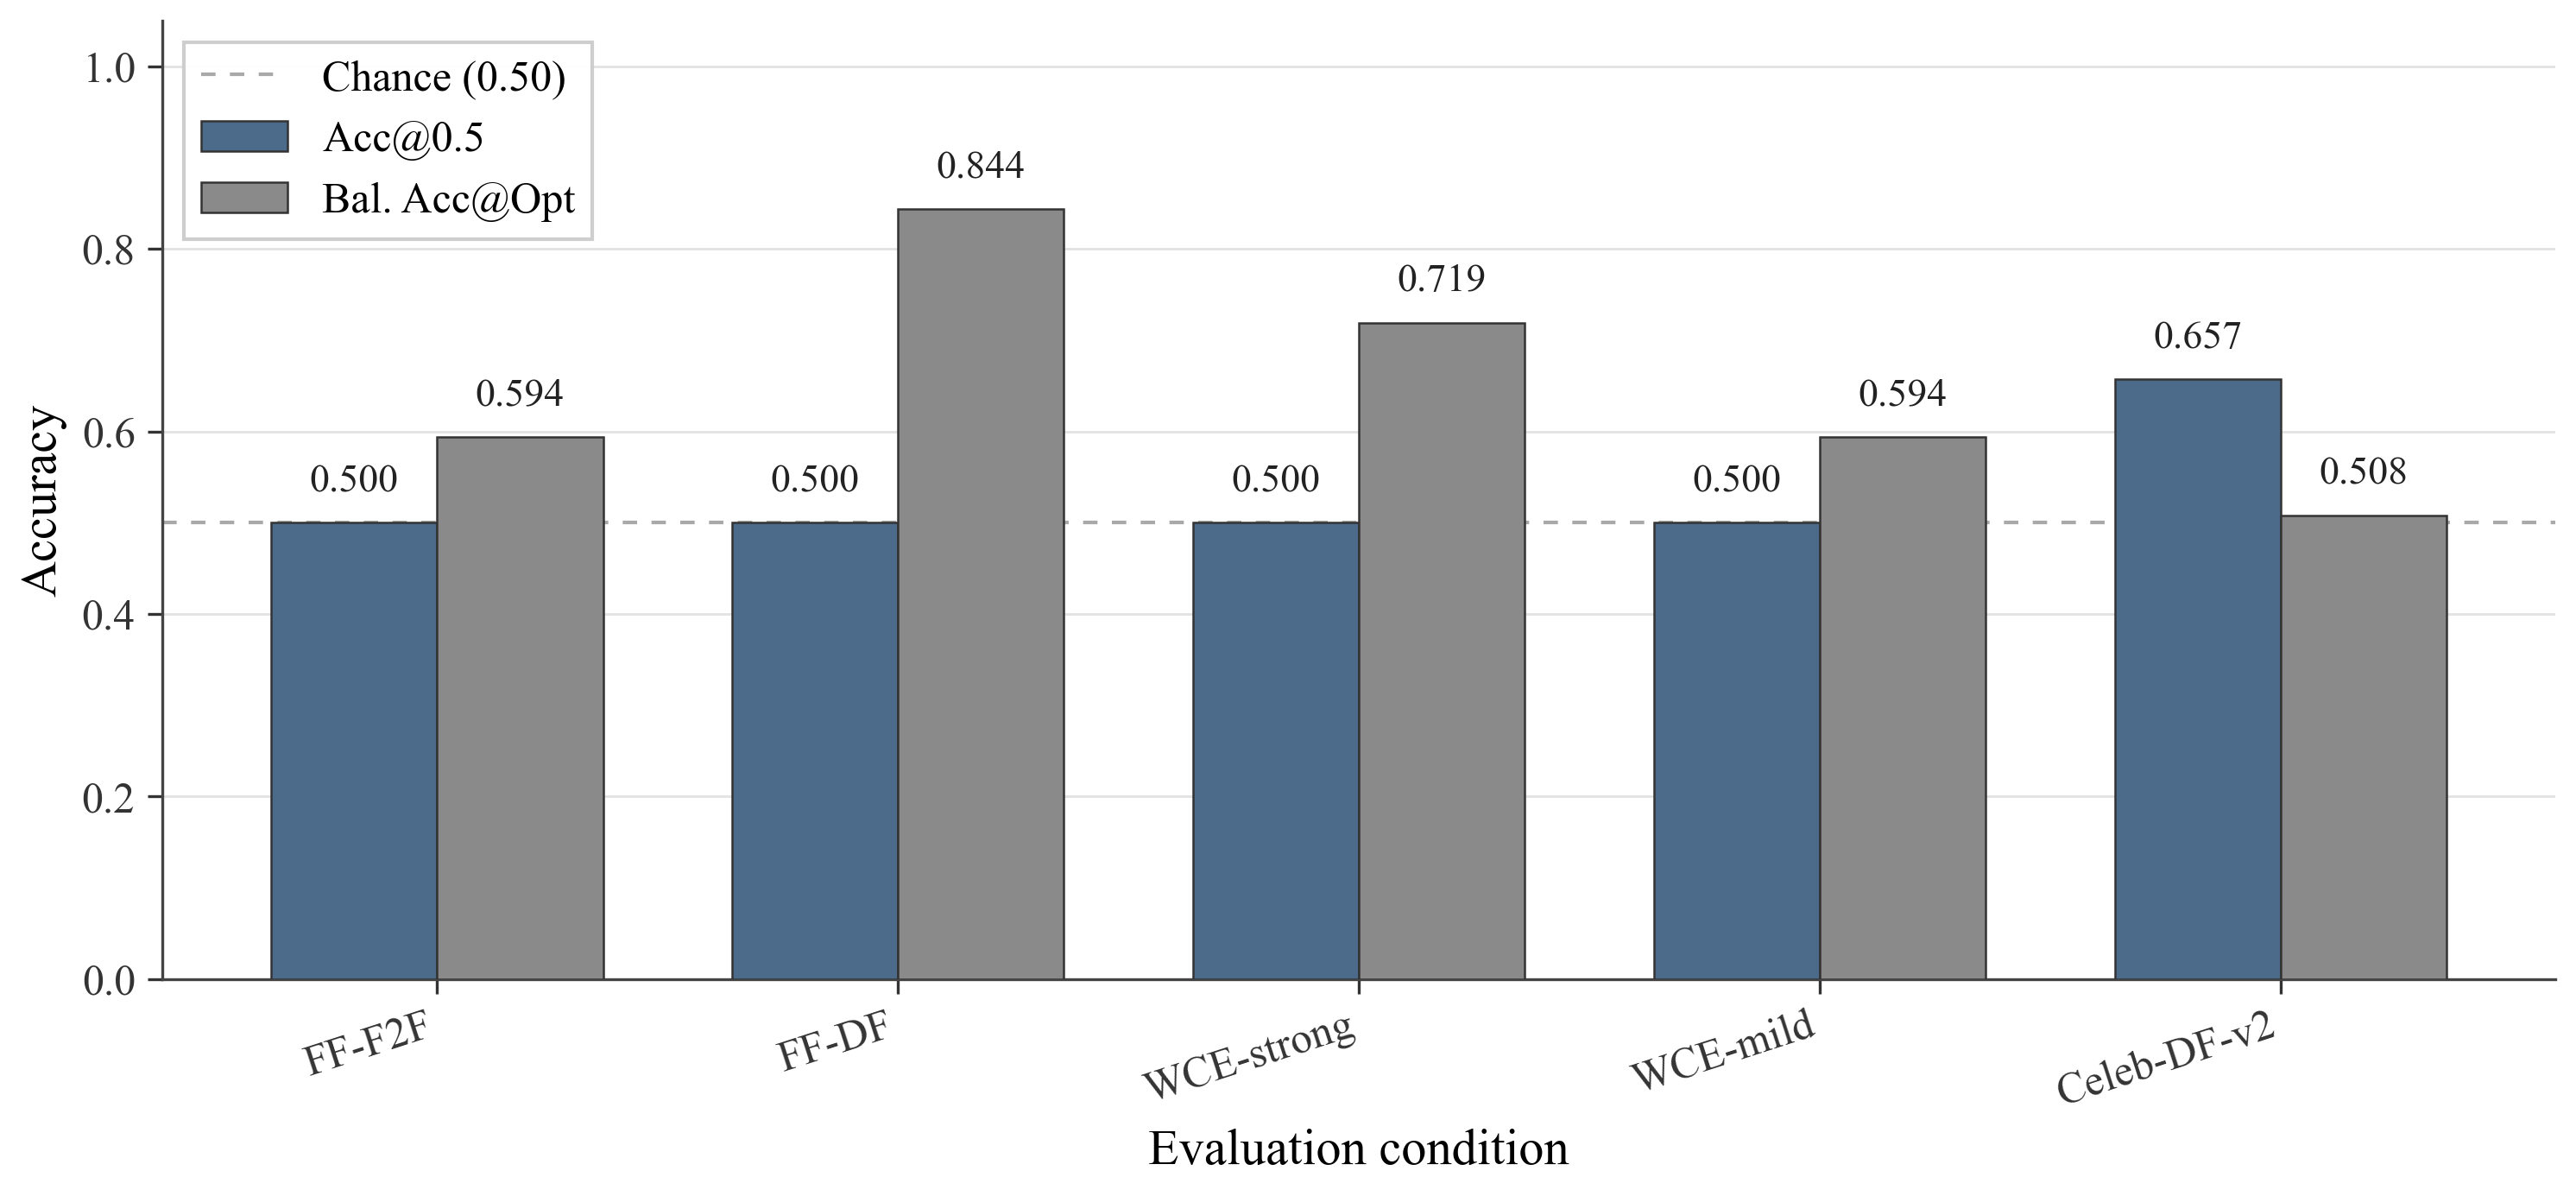
\includegraphics[width=\linewidth]{fig_threshold_comparison.png}
  \caption{Acc@0.5 versus balanced accuracy at the ROC-optimal threshold (Bal.~Acc@Opt). The dashed line denotes chance (0.50). A large gap on FF-DF indicates threshold collapse with preserved ranking; on Celeb-DF-v2 both metrics remain near chance.}
  \label{fig:threshold_comparison}
\end{figure}


\section{In-Distribution Behaviour}
\label{sec:indist}

Both in-distribution conditions produce AUC near random:
0.550 for scratch initialisation and 0.526 for pretrained
fine-tuning.
At threshold~0.5, both predict fake for nearly all samples,
yielding approximately 50\% accuracy and zero real-class
recall.

These results are weak and should be interpreted with
caution.
Training for two epochs with batch size~4 is substantially
below the convergence requirements for this model on FF++.
Standard fully-trained Xception baselines in the literature
typically reach AUC above 0.99 on FF++ in-distribution
and AUC in the range 0.65--0.75 on Celeb-DF-v2 under
cross-dataset evaluation~\cite{deepfakebench}.
The in-distribution results here therefore reflect
training insufficiency rather than model incapacity.

Their value in this study is not as a performance claim
but as a starting observation: the consistent class-collapse
at threshold~0.5 across both in-distribution conditions
directly motivates the threshold-aware analysis protocol
adopted throughout.
If the detector had produced balanced predictions at 0.5
from the outset, the question of threshold behaviour
under distribution shift would not have arisen in the
same form.
The consequence for the cross-manipulation and external
conditions is also important to state directly.
If the baseline had converged, AUC on those conditions
would likely be higher, and the threshold dynamics might
differ in magnitude.
We therefore present the threshold analysis as a
characterisation of the specific operating point produced
by this training regime, not as a general claim about
Xception behaviour.
The conceptual distinction between threshold collapse and
ranking degradation, however, does not depend on the
absolute level of AUC; it depends only on the relationship
between AUC and thresholded performance, which is
observable regardless of training strength.

\section{Internal Shift: FF-F2F and FF-DF}
\label{sec:internal}

The two cross-manipulation conditions tell different
stories, and the difference is instructive.
Even within the same benchmark family, internal
distribution shift is not uniform: some manipulation
types remain partially rank-separable while others
do not, and this distinction is not visible from
in-distribution performance alone.

On FF-F2F, AUC is 0.547 and balanced accuracy at the
optimal threshold is 0.594.
Both measures are close to chance.
The detector does not retain useful discriminative signal
when transferred to Face2Face manipulation, suggesting
that whatever artifacts it learned during training do not
transfer to this manipulation type.
This condition corresponds to a mild form of ranking
degradation.

On FF-DF, the picture changes substantially.
AUC reaches 0.793, indicating genuine ranking ability.
At the default threshold of 0.5, however, the detector
still predicts fake for almost all samples, producing
near-random classification.
The threshold analysis resolves this apparent
contradiction: at a threshold of 0.736, balanced accuracy
rises to 0.844.
As shown in Table~\ref{tab:classwise}, this threshold
yields perfect real-class accuracy (1.000) and 0.688
fake-class accuracy.

This is the central empirical finding of the project.
The model is not broken on FF-DF in any representational
sense---its predictions, as rankings, are substantially
correct.
The failure is that the score distribution has shifted
relative to the training distribution: the mass of
predicted probabilities sits higher than it did during
training, making threshold~0.5 too conservative.
A practitioner deploying this detector at threshold~0.5
would observe near-random classification on FF-DF
face-swaps despite the model having AUC~0.793.
This failure is entirely attributable to threshold
miscalibration, not model collapse---and it is in
principle recoverable through post-hoc
calibration~\cite{aigicalib2025,calibration2025}.

\begin{figure}[t]
  \centering
  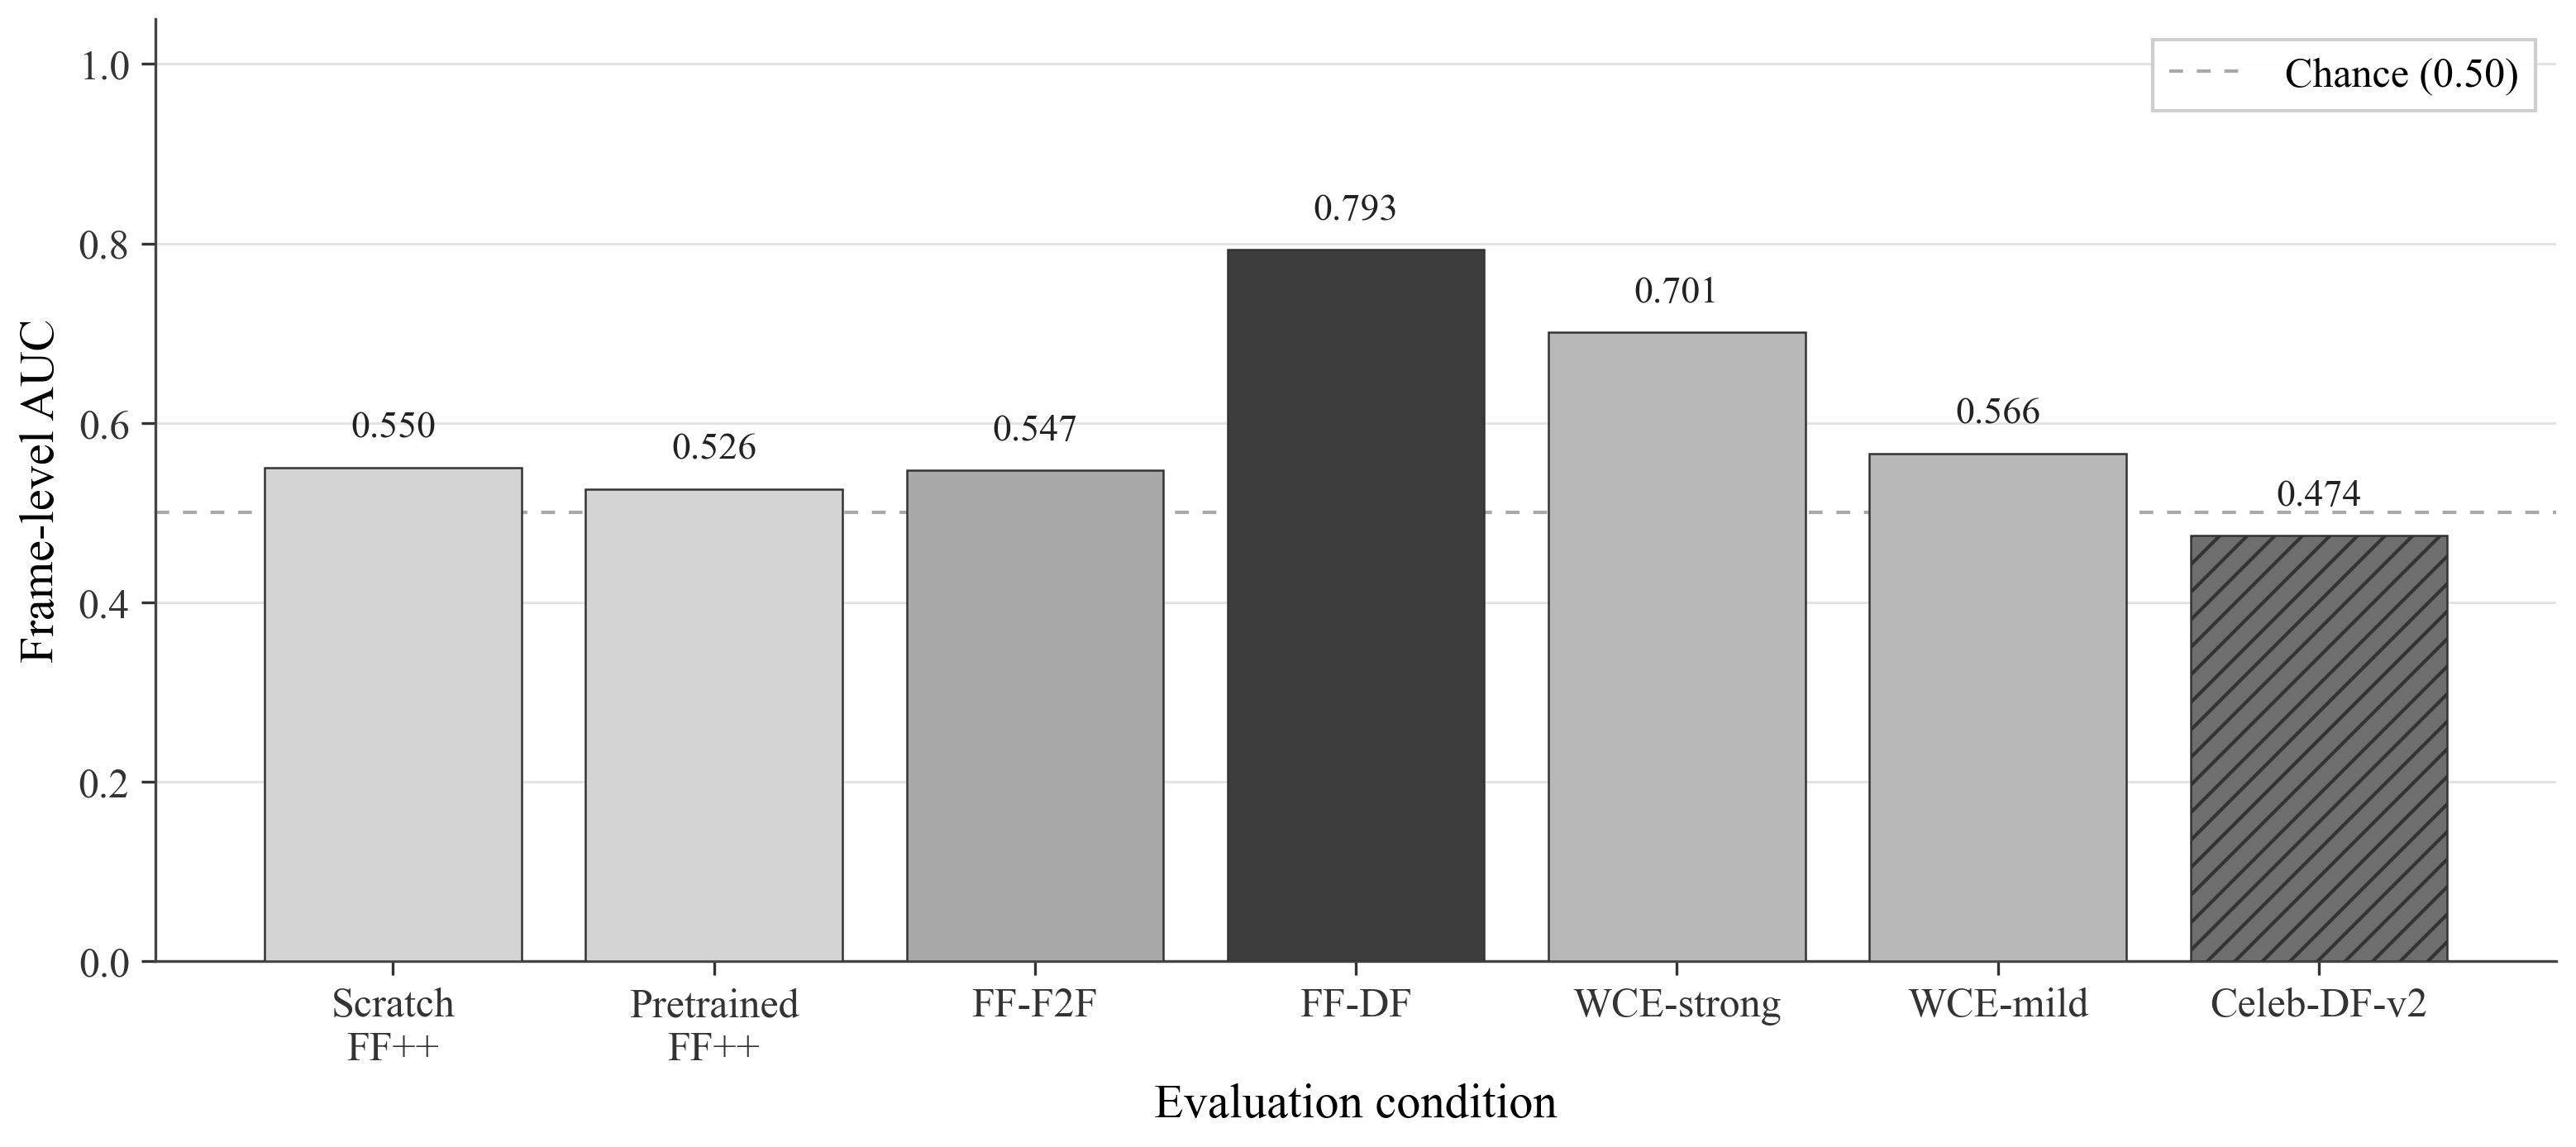
\includegraphics[width=\linewidth]{fig_auc_comparison.png}
  \caption{Frame-level AUC by evaluation condition (chance = 0.50, dashed). FF-DF retains strong internal ranking (AUC~=~0.793); Celeb-DF-v2 falls below chance (AUC~=~0.474), indicating cross-dataset ranking degradation.}
  \label{fig:auc_comparison}
\end{figure}

\section{Weighted Cross-Entropy Experiments}
\label{sec:wce}

Both WCE conditions are evaluated on FF-DF for direct
comparison against the baseline.
The rationale for the experiment is the following: if
the threshold collapse on FF-DF is caused by insufficient
penalty on fake-class errors during training, then
upweighting the fake class in the loss should strengthen
the model's response to fake samples and potentially
shift the score distribution, bringing the effective
threshold closer to 0.5.

The results do not support this hypothesis.
The strong weighting ($[2.0, 1.0]$) reduces AUC from
0.793 to 0.701 and reduces fake-class accuracy at the
optimal threshold from 0.688 to 0.438, without improving
real-class accuracy.
The mild weighting ($[1.5, 1.0]$) gives AUC of 0.566
and balanced accuracy of 0.594, both substantially below
the baseline.
Neither setting produces a threshold near 0.5: the
WCE-strong optimal threshold is 0.516 (only slightly
shifted from 0.5) and WCE-mild is 0.527.
In both cases, the threshold shift does not translate
into improved balanced accuracy.

This is a useful negative result.
Threshold collapse on FF-DF is not explained by a
fake-class penalty effect that can be corrected at the
loss level.
The mechanism is better described as a shift in the
overall shape of the score distribution between the
training and test conditions---a score calibration
problem rather than a training-objective problem.
This diagnosis points toward the appropriate class of
remediation: post-hoc calibration methods such as
temperature scaling or Platt scaling, which directly
adjust the score distribution rather than the training
objective~\cite{aigicalib2025}.

\section{External Evaluation: Celeb-DF-v2}
\label{sec:external}

The external evaluation on Celeb-DF-v2 reveals a
qualitatively different failure mode from FF-DF.

AUC is 0.474, which is below the random baseline of 0.5.
This indicates that ranking quality has degraded
substantially: the detector's predicted scores are no
longer meaningfully ordered with respect to ground truth,
and performance becomes effectively near-random as a
ranking.
At the default threshold of 0.5, accuracy appears
relatively high (0.657), but this is not a meaningful
result: as shown in Table~\ref{tab:classwise},
real-class accuracy at the optimal threshold is 0.070
and fake-class accuracy is 0.945, meaning the detector
is classifying nearly everything as fake.
The apparent Acc@0.5 is inflated by the class distribution
of the test set, not by any genuine discrimination.
Balanced accuracy at the optimal threshold is 0.508,
effectively random.

This failure is not threshold collapse.
The detector's rankings are not informative, so adjusting
the threshold does not help: there is no ``good'' threshold
because the scores carry no signal about the true label.
This is ranking degradation---a more severe failure mode
that reflects the model's inability to generalise its
learned features to the Celeb-DF-v2 distribution.

The contrast with FF-DF is the central interpretive
finding of this project.
On FF-DF, AUC~=~0.793 and calibration can recover
performance.
On Celeb-DF-v2, AUC~=~0.474 and calibration cannot help.
Two conditions that both look like ``generalisation failure''
at threshold~0.5 are in fact two different failures with
different causes and different remedies.
Threshold-aware analysis makes this distinction visible;
AUC alone does not.

% ============================================================
\chapter{Discussion}
% ============================================================

\section{Two Failure Modes and Their Implications}

The main conceptual contribution of this project is the
operationalisation of two failure modes that deepfake
detector evaluations typically conflate.

\textbf{Threshold collapse} is characterised by AUC
substantially above 0.5 combined with near-random
performance at threshold 0.5.
The mechanism is a shift in the model's score distribution
at test time: the relative ordering of predictions is
preserved, but the absolute positions of the scores
move.
This failure is in principle recoverable.
If a small calibration set from the target distribution
is available, methods such as temperature scaling,
Platt scaling, or the Bayesian logit correction
of~\cite{aigicalib2025} can realign the decision boundary
without retraining the backbone.
Our results provide the empirical motivation for why
such calibration is necessary: a model with AUC~0.793
on FF-DF produces near-random classification at the
default threshold, purely because the threshold is wrong.

\textbf{Ranking degradation} is characterised by AUC
near or below 0.5.
The model's score function is not informative as a
ranking, so no threshold can recover meaningful
classification.
This failure requires better generalisation at the
representation level---the kind of improvement that
methods like LSDA~\cite{lsda2024},
P\&P~\cite{p_and_p2025}, and related
approaches~\cite{gend2025} pursue through improved
training procedures and architectural design.
Post-hoc calibration is irrelevant to this failure mode.

The practical importance of distinguishing these two
failure modes lies in the selection of remediation
strategy.
A system that exhibits threshold collapse but not
ranking degradation is a potentially viable detector
that needs calibration at deployment time.
A system that exhibits ranking degradation cannot be
salvaged by calibration alone.
Conflating the two---as a single AUC number or a single
fixed-threshold accuracy would---leads to different
misdiagnoses.
If threshold collapse is misread as ranking degradation,
a working detector may be discarded unnecessarily.
If ranking degradation is misread as threshold collapse,
resources may be spent on calibration that will not work.
More broadly, not every apparent failure under distribution
shift requires the same remedy: conditions that preserve
ranking ability primarily require calibration at
deployment time, while conditions that exhibit ranking
degradation require improvements at the representation
level---better training objectives, more diverse data, or
more generalisable architectures.

\section{Why Weighted Cross-Entropy Does Not Help}

The failure of both WCE experiments is informative beyond
simply ruling out a hypothesis.
It demonstrates that the threshold-collapse pattern on
FF-DF is robust to a simple training-time intervention
that directly increases the penalty on fake-class errors.
Both weight settings reduce fake-class accuracy at the
optimal threshold without improving balanced accuracy,
suggesting a trade-off rather than a genuine improvement.

This is consistent with the interpretation that threshold
collapse is a test-time distribution shift effect rather
than a training-set effect.
The model's score distribution shifts at test time because
the features it has learned do not produce the same
discriminative signal on FF-DF that they produced on FF++.
Changing the loss weights during training does not change
what features the model learns or how the score
distribution behaves at test time.
What is required is an intervention that acts on the
score distribution after the model is applied---which
is precisely what calibration methods do.

\section{Limitations}
\label{sec:limitations}

Several limitations should be stated clearly.

\textbf{Underpowered training.}
Two epochs with batch size~4 is insufficient for stable
Xception convergence on FF++.
The in-distribution AUC values near 0.5 are a direct
consequence.
The cross-manipulation and external results are also
affected: a fully converged baseline would likely show
higher AUC on FF-DF and might show different threshold
dynamics.
The results are therefore descriptive of this specific
training regime, not necessarily representative of
Xception behaviour in general.

\textbf{Optimistic threshold selection.}
The optimal threshold is selected on the evaluation set
itself by maximising F1.
In a real deployment setting, the threshold must be
fixed before test data is seen, using a separate
calibration set or a prior from the training
distribution.
The Bal.~Acc@Opt values are therefore upper bounds on
what a deployed system could achieve through
threshold selection alone, without access to target
distribution data.

\textbf{Single backbone.}
Only Xception is studied.
The threshold-collapse pattern may look different for
models with different output calibration properties,
or for models trained with stronger regularisation.

\textbf{Small evaluation sets.}
Some conditions involve small numbers of samples,
which limits the statistical reliability of the
reported metrics.

\textbf{No calibration experiment.}
The logical next step after identifying threshold
collapse would be to apply a post-hoc calibration
method (e.g.\ temperature scaling) on a small
held-out calibration split and measure recovery.
This was not conducted within the scope of this project.

% ============================================================
\chapter{Conclusion}
% ============================================================

This report has studied how a standard deepfake detector
fails under distribution shift, with particular attention
to the decision threshold.
Using the Xception baseline in DeepfakeBench, trained on
FaceForensics++ and evaluated across internal and external
shift conditions, the study identifies and characterises
two qualitatively distinct failure modes.

\textbf{Threshold collapse} (FF-DF): the model retains
ranking ability (AUC~=~0.793) but the score distribution
shifts under distribution shift, causing the default
threshold to become miscalibrated.
Classification at threshold~0.5 is near-random; balanced
accuracy recovers to 0.844 at an optimised threshold of
0.736.
This failure is in principle recoverable through
post-hoc calibration methods.

\textbf{Ranking degradation} (Celeb-DF-v2): the model's
score function is no longer informative as a ranking
(AUC~=~0.474).
Threshold adjustment provides no recovery; balanced
accuracy at the optimal threshold is 0.508, effectively
random.
This failure requires improved generalisation at the
representation level.

Weighted cross-entropy experiments on FF-DF confirm that
neither failure mode is attributable to a fake-class
penalty effect in the loss, pointing to score distribution
shift as the causal mechanism for threshold collapse and
motivating calibration-based remediation.

The central practical takeaway is direct: a practitioner
who trains on FF++ and deploys at threshold~0.5 will
observe near-random classification on FF-DF face-swaps
despite the model having AUC~0.793.
AUC alone does not reveal this, because AUC does not
depend on the threshold.
Threshold-aware analysis makes the failure visible and,
crucially, makes it possible to distinguish between
failures that calibration can fix and failures that it
cannot.

\subsection*{Future Work}

The most immediate extension of this work is a post-hoc
calibration experiment on the FF-DF threshold-collapse
condition.
Temperature scaling or Platt scaling applied to a small
calibration split from the FF-DF distribution---or the
Bayesian logit correction of Yang~et~al.~\cite{aigicalib2025}---would
directly test whether the AUC-0.793 ranking ability can
be translated into strong thresholded performance through
calibration alone.
A converged training run would also strengthen the study
by providing a more reliable baseline from which to
measure distribution shift effects.
Further work could extend the threshold analysis to
additional backbones and datasets, and could examine
whether training methods designed for cross-distribution
generalisation~\cite{lsda2024,p_and_p2025,gend2025}
also reduce threshold collapse, or primarily improve
ranking quality.

% ============================================================
% BIBLIOGRAPHY
% ============================================================
\begin{thebibliography}{99}

\bibitem{rossler2019}
A.~Rossler, D.~Cozzolino, L.~Verdoliva, C.~Riess,
J.~Thies, and M.~Nie{\ss}ner,
``FaceForensics++: Learning to Detect Manipulated Facial
Images,''
in \textit{Proc.\ ICCV}, 2019.

\bibitem{chollet2017}
F.~Chollet,
``Xception: Deep Learning with Depthwise Separable
Convolutions,''
in \textit{Proc.\ CVPR}, 2017.

\bibitem{li2020celebdf}
Y.~Li, X.~Yang, P.~Sun, H.~Qi, and S.~Lyu,
``Celeb-DF: A Large-Scale Challenging Dataset for
DeepFake Forensics,''
in \textit{Proc.\ CVPR}, 2020.

\bibitem{deepfakebench}
Z.~Yan, Y.~Zhang, X.~Yuan, S.~Lyu, and B.~Wu,
``DeepfakeBench: A Comprehensive Benchmark of Deepfake
Detection,''
in \textit{Advances in Neural Information Processing
Systems (NeurIPS)}, 2023.

\bibitem{tolosana2020}
R.~Tolosana, R.~Vera-Rodriguez, J.~Fierrez,
A.~Morales, and J.~Ortega-Garcia,
``DeepFakes and Beyond: A Survey of Face Manipulation
and Fake Detection,''
\textit{Information Fusion}, vol.~64,
pp.~131--148, 2020.

\bibitem{gend2025}
A.~Yermakov, J.~Cech, J.~Matas, and M.~Fritz,
``Deepfake Detection that Generalizes Across Benchmarks,''
\textit{arXiv:2508.06248}, 2025.

\bibitem{aigicalib2025}
M.~Yang et al.,
``Your AI-Generated Image Detector Can Secretly Achieve
SOTA Accuracy, If Calibrated,''
in \textit{Proc.\ AAAI}, 2026.

\bibitem{calibration2025}
Y.~Zhang et al.,
``Towards Reliable Deepfake Detection from an Uncertainty
Calibration Perspective,''
\textit{Visual Intelligence}, 2025.

\bibitem{lsda2024}
Z.~Yan, Y.~Luo, S.~Lyu, Q.~Liu, and B.~Wu,
``Transcending Forgery Specificity with Latent Space
Augmentation for Generalizable Deepfake Detection,''
in \textit{Proc.\ CVPR}, 2024.

\bibitem{p_and_p2025}
Z.~Yan et al.,
``Generalizing Deepfake Video Detection with Plug-and-Play:
Video-Level Blending and Spatiotemporal Adapter Tuning,''
in \textit{Proc.\ CVPR}, 2025.

\bibitem{d3_2025}
Y.~Yang et al.,
``D$^3$: Scaling Up Deepfake Detection by Learning from
Discrepancy,''
in \textit{Proc.\ CVPR}, 2025.

\end{thebibliography}

\end{document}